% HW2 high dimensional data

\documentclass[12pt, leqno]{article}\usepackage[]{graphicx}\usepackage[]{color}
%% maxwidth is the original width if it is less than linewidth
%% otherwise use linewidth (to make sure the graphics do not exceed the margin)
\makeatletter
\def\maxwidth{ %
  \ifdim\Gin@nat@width>\linewidth
    \linewidth
  \else
    \Gin@nat@width
  \fi
}
\makeatother

\definecolor{fgcolor}{rgb}{0.345, 0.345, 0.345}
\newcommand{\hlnum}[1]{\textcolor[rgb]{0.686,0.059,0.569}{#1}}%
\newcommand{\hlstr}[1]{\textcolor[rgb]{0.192,0.494,0.8}{#1}}%
\newcommand{\hlcom}[1]{\textcolor[rgb]{0.678,0.584,0.686}{\textit{#1}}}%
\newcommand{\hlopt}[1]{\textcolor[rgb]{0,0,0}{#1}}%
\newcommand{\hlstd}[1]{\textcolor[rgb]{0.345,0.345,0.345}{#1}}%
\newcommand{\hlkwa}[1]{\textcolor[rgb]{0.161,0.373,0.58}{\textbf{#1}}}%
\newcommand{\hlkwb}[1]{\textcolor[rgb]{0.69,0.353,0.396}{#1}}%
\newcommand{\hlkwc}[1]{\textcolor[rgb]{0.333,0.667,0.333}{#1}}%
\newcommand{\hlkwd}[1]{\textcolor[rgb]{0.737,0.353,0.396}{\textbf{#1}}}%

\usepackage{framed}
\makeatletter
\newenvironment{kframe}{%
 \def\at@end@of@kframe{}%
 \ifinner\ifhmode%
  \def\at@end@of@kframe{\end{minipage}}%
  \begin{minipage}{\columnwidth}%
 \fi\fi%
 \def\FrameCommand##1{\hskip\@totalleftmargin \hskip-\fboxsep
 \colorbox{shadecolor}{##1}\hskip-\fboxsep
     % There is no \\@totalrightmargin, so:
     \hskip-\linewidth \hskip-\@totalleftmargin \hskip\columnwidth}%
 \MakeFramed {\advance\hsize-\width
   \@totalleftmargin\z@ \linewidth\hsize
   \@setminipage}}%
 {\par\unskip\endMakeFramed%
 \at@end@of@kframe}
\makeatother

\definecolor{shadecolor}{rgb}{.97, .97, .97}
\definecolor{messagecolor}{rgb}{0, 0, 0}
\definecolor{warningcolor}{rgb}{1, 0, 1}
\definecolor{errorcolor}{rgb}{1, 0, 0}
\newenvironment{knitrout}{}{} % an empty environment to be redefined in TeX

\usepackage{alltt}
\usepackage{amsfonts, amsmath, amssymb}
\usepackage{amsthm}
\usepackage{mathtools}
\usepackage{fancyhdr}
\usepackage{hyperref}
\usepackage{graphicx}
\usepackage{caption}
\usepackage{subcaption}
\usepackage{float}
\usepackage{mathrsfs}
\usepackage{array} 
\usepackage{rotating}
%\usepackage{babel}
\providecommand{\abs}[1]{\lvert#1\rvert}
\providecommand{\norm}[1]{\lVert#1\rVert}
\newcommand{\macheps}{\epsilon_{\mbox{\scriptsize mach}}}
\let\oldhat\hat
\renewcommand{\vec}[1]{\mathbf{#1}}
\renewcommand{\hat}[1]{\oldhat{{#1}}}
\def\rp{\ensuremath \mathbb{R}^p}
\def\rpp{\ensuremath \mathbb{R}^{p \times p}}
\def\s{\ensuremath\Sigma}
\def\om{\ensuremath\Omega}
\def\pd{\ensuremath\mathbb{P}^+}
\def\pg{\ensuremath\mathbb{P}_{{G}}}
\def\E{\ensuremath\mathbb{E}}
\def\normdist[#1]#2{\ensuremath \sim \mathcal{N} (#1,#2) }
\def\ndist1{\ensuremath \sim \mathcal{N}  (\mu, \sigma)}
\def\ndistvec{\ensuremath \sim \mathcal{N}_p ( {\mu},  {\Sigma})}
\def\lra{\ensuremath\Leftrightarrow}
\def\stackrel#1#2{\mathrel{\mathop{#2}\limits^{#1}}}
\newcommand\ind{\protect\mathpalette{\protect\independenT}{\perp}}
\def\independenT#1#2{\mathrel{\rlap{$#1#2$}\mkern2mu{#1#2}}}
\makeatletter
\newtheorem{thm}{Theorem}[]
\newtheorem{lemma}{Lemma}[]
\newtheorem{defn}[thm]{Definition}
\newcommand{\sign}{\mathrm{sign}}
\newcommand{\distas}[1]{\mathbin{\overset{#1}{\kern\z@\sim}}}%
\newsavebox{\mybox}\newsavebox{\mysim}
\newcommand{\dist}[1]{%
  \savebox{\mybox}{\hbox{\kern3pt$\scriptstyle#1$\kern3pt}}%
  \savebox{\mysim}{\hbox{$\sim$}}%
  \mathbin{\overset{#1}{\kern\z@\resizebox{\wd\mybox}{\ht\mysim}{$\sim$}}}%
}
\makeatother

\IfFileExists{upquote.sty}{\usepackage{upquote}}{}
\begin{document}

<style type="text/css">

body, td {
   font-size: 12px;
}
code.r{
  font-size: 12px;
}
pre {
  font-size: 12px
}
</style>
\pagestyle{fancy}
\lhead{Syed Rahman}
\rhead{STA6707}

\begin{center}
{\large {\bf Homework 2 - Solutions to Homework 1}} \\
{\it{Syed Rahman}} \\
\end{center}

\paragraph{Problem 1:}

The data set USTATES-data.txt (available in the folder Data Sets) contains the unemployment rates of the 50 US States, plus those of the District of Columbia and Puerto Rico for the period Jan 1976- March 2007.
Use PCA analysis to summarize the basic patterns in the data and carefully comment on the results.
Specifically, discuss in your report possible transformations of the variables, exclusion of outliers, choice of number of principal components, fit of the solution, interpretation of the principal components.

\paragraph{Solution 1:}
In this problem, we note that $p >> n$. One approach is to
transpose the data, however, this is ultimately incorrect as it would
be harder to justify the $X_i \stackrel{iid}{\sim} \mathcal{N}_p (
{\mu},  {\Sigma})$ assumption of PCA. Instead we use an SVD based function to
perform PCA. Doing the analysis with and without PR in addition to the
following in Figures \ref{fig:p1a} and \ref{fig:p1b} indicates that it is an outlier and that it should be left out of the final analysis. 
\begin{knitrout}
\definecolor{shadecolor}{rgb}{0.969, 0.969, 0.969}\color{fgcolor}\begin{kframe}
\begin{alltt}
\hlstd{data1} \hlkwb{=} \hlkwd{read.table}\hlstd{(}\hlstr{"USTATES-data-1.txt"}\hlstd{,} \hlkwc{header}\hlstd{=}\hlnum{TRUE}\hlstd{)}
\hlstd{data0} \hlkwb{=} \hlkwd{as.matrix}\hlstd{(data1)}
\hlstd{pc1} \hlkwb{=} \hlkwd{prcomp}\hlstd{(data0,} \hlkwc{center} \hlstd{=} \hlnum{TRUE}\hlstd{)}
\hlkwd{summary}\hlstd{(pc1)}\hlopt{$}\hlstd{importance[,}\hlnum{1}\hlopt{:}\hlnum{4}\hlstd{]}
\end{alltt}
\begin{verbatim}
##                             PC1      PC2      PC3      PC4
## Standard deviation     35.49366 12.66850 8.843756 5.704322
## Proportion of Variance  0.76815  0.09786 0.047690 0.019840
## Cumulative Proportion   0.76815  0.86601 0.913700 0.933540
\end{verbatim}
\end{kframe}
\end{knitrout}
\begin{knitrout}
\definecolor{shadecolor}{rgb}{0.969, 0.969, 0.969}\color{fgcolor}\begin{kframe}
\begin{alltt}
\hlkwd{matplot}\hlstd{(}\hlkwd{t}\hlstd{(data0),}\hlkwc{type} \hlstd{=} \hlstr{"l"}\hlstd{,} \hlkwc{xlab} \hlstd{=} \hlstr{"Years"}\hlstd{,} \hlkwc{ylab} \hlstd{=} \hlstr{"Unemployment Rates"}\hlstd{)}
\end{alltt}
\end{kframe}\begin{figure}[H]
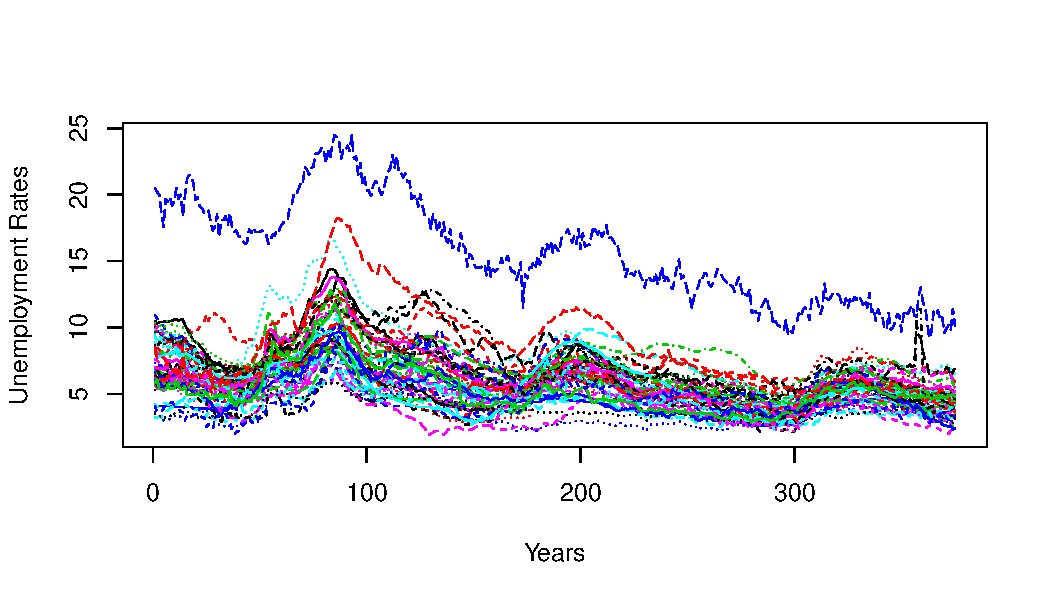
\includegraphics[width=\maxwidth]{figure/p1a-1} \caption[Unemployment Rates by state]{Unemployment Rates by state}\label{fig:p1a}
\end{figure}


\end{knitrout}
\begin{knitrout}
\definecolor{shadecolor}{rgb}{0.969, 0.969, 0.969}\color{fgcolor}\begin{kframe}
\begin{alltt}
\hlkwd{plot}\hlstd{(pc1}\hlopt{$}\hlstd{x[,}\hlnum{1}\hlstd{],pc1}\hlopt{$}\hlstd{x[,}\hlnum{2}\hlstd{] ,} \hlkwc{xlab}\hlstd{=}\hlstr{"PC1"}\hlstd{,}\hlkwc{ylab}\hlstd{=}\hlstr{"PC2"}\hlstd{,}\hlkwc{type}\hlstd{=}\hlstr{"n"}\hlstd{,}\hlkwc{lwd}\hlstd{=}\hlnum{2}\hlstd{)}
\hlkwd{text}\hlstd{(pc1}\hlopt{$}\hlstd{x[,}\hlnum{1}\hlstd{],pc1}\hlopt{$}\hlstd{x[,}\hlnum{2}\hlstd{],}\hlkwc{labels}\hlstd{=}\hlkwd{abbreviate}\hlstd{(}\hlkwd{row.names}\hlstd{(data1)),}\hlkwc{cex}\hlstd{=}\hlnum{0.7}\hlstd{,}\hlkwc{lwd}\hlstd{=}\hlnum{2}\hlstd{)}
\end{alltt}
\end{kframe}\begin{figure}[H]
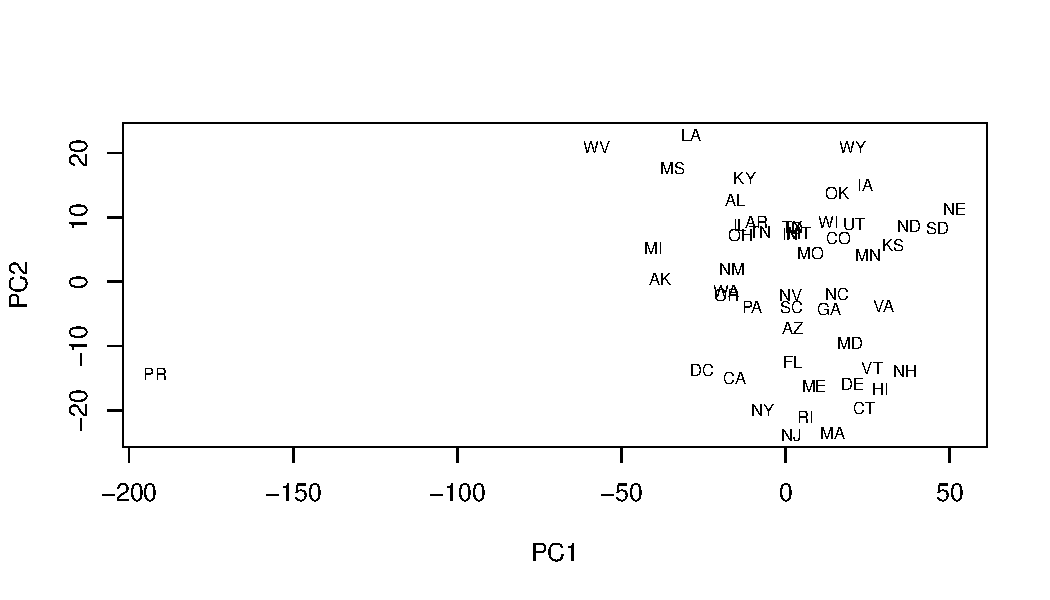
\includegraphics[width=\maxwidth]{figure/p1b-1} \caption[Bi-plot including PR]{Bi-plot including PR}\label{fig:p1b}
\end{figure}


\end{knitrout}
\begin{knitrout}
\definecolor{shadecolor}{rgb}{0.969, 0.969, 0.969}\color{fgcolor}\begin{kframe}
\begin{alltt}
\hlstd{data} \hlkwb{=} \hlstd{data0[}\hlopt{-}\hlnum{40}\hlstd{,]}
\hlstd{pc2} \hlkwb{=} \hlkwd{prcomp}\hlstd{(data,} \hlkwc{center} \hlstd{=} \hlnum{TRUE}\hlstd{)}
\hlkwd{summary}\hlstd{(pc2)}\hlopt{$}\hlstd{importance[,}\hlnum{1}\hlopt{:}\hlnum{4}\hlstd{]}
\end{alltt}
\begin{verbatim}
##                             PC1      PC2      PC3      PC4
## Standard deviation     23.32671 12.33142 8.861459 5.608603
## Proportion of Variance  0.59591  0.16653 0.086000 0.034450
## Cumulative Proportion   0.59591  0.76244 0.848440 0.882880
\end{verbatim}
\end{kframe}
\end{knitrout}
The screeplot in Figure \ref{fig:p1d} indicates that it is sufficient to hold on to 2 PCs.
\begin{knitrout}
\definecolor{shadecolor}{rgb}{0.969, 0.969, 0.969}\color{fgcolor}\begin{kframe}
\begin{alltt}
\hlkwd{screeplot}\hlstd{(pc2)}
\end{alltt}
\end{kframe}\begin{figure}[H]
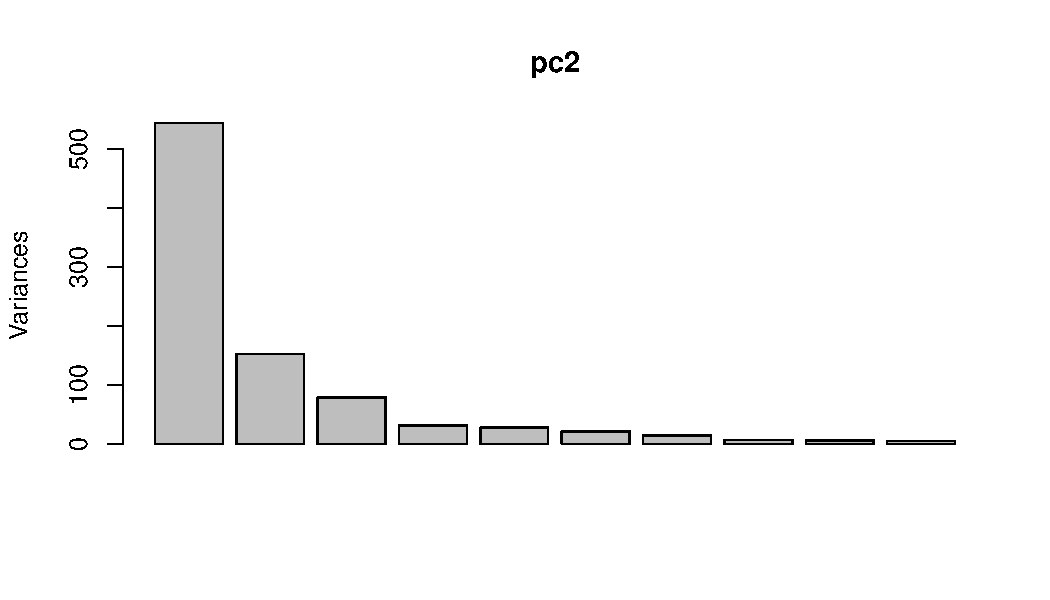
\includegraphics[width=\maxwidth]{figure/p1d-1} \caption[Screeplot excluding PR]{Screeplot excluding PR}\label{fig:p1d}
\end{figure}


\end{knitrout}

Finally, taking a look at the factor loadings in addition to look at
the bi-plot in Figure \ref{fig:p1e} suggest that PC1 is essentially an
average of all the months, while PC2 is positive over certain time
time periods while negative over others. In additon, the variables are
all very closely related to each other due to the small angles between
them on the bi-plot.
\begin{knitrout}
\definecolor{shadecolor}{rgb}{0.969, 0.969, 0.969}\color{fgcolor}\begin{kframe}
\begin{alltt}
\hlkwd{biplot}\hlstd{(pc2)}
\end{alltt}
\end{kframe}\begin{figure}[H]
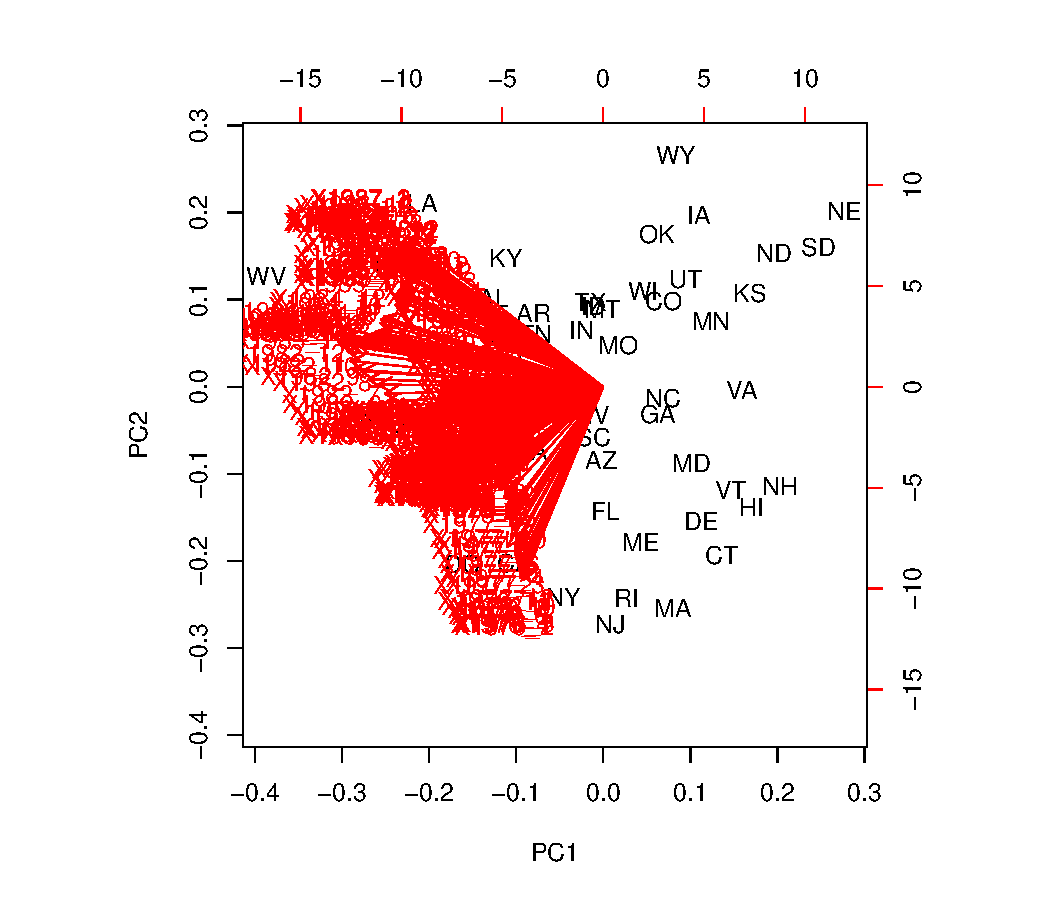
\includegraphics[width=\maxwidth]{figure/p1e-1} \caption[Bi-plot excluding PR]{Bi-plot excluding PR}\label{fig:p1e}
\end{figure}


\end{knitrout}

To check the fit of the data we do a simple bootstrap and estimate the
proportion of data explained by 2 variables. The center of
the histogram is near 0.76, which indicates that the PCA is a good fit
for the data.
\begin{knitrout}
\definecolor{shadecolor}{rgb}{0.969, 0.969, 0.969}\color{fgcolor}\begin{kframe}
\begin{alltt}
\hlkwd{set.seed}\hlstd{(}\hlnum{12345}\hlstd{)}
\hlstd{niter} \hlkwb{=} \hlnum{1000}
\hlstd{propexp} \hlkwb{=} \hlkwd{matrix}\hlstd{(}\hlnum{0}\hlstd{,}\hlnum{1000}\hlstd{,}\hlnum{1}\hlstd{);}
\hlkwa{for}\hlstd{(i} \hlkwa{in} \hlnum{1}\hlopt{:}\hlnum{1000}\hlstd{)\{}
   \hlstd{pc} \hlkwb{=} \hlkwd{prcomp}\hlstd{(data[}\hlkwd{sample}\hlstd{(}\hlkwd{nrow}\hlstd{(data),}\hlkwc{size}\hlstd{=}\hlnum{51}\hlstd{,}\hlkwc{replace}\hlstd{=}\hlnum{TRUE}\hlstd{),])}
   \hlstd{propexp[i,}\hlnum{1}\hlstd{]} \hlkwb{=} \hlkwd{sum}\hlstd{(pc}\hlopt{$}\hlstd{sdev[}\hlnum{1}\hlopt{:}\hlnum{2}\hlstd{]}\hlopt{^}\hlnum{2}\hlstd{)}\hlopt{/}\hlkwd{sum}\hlstd{(pc}\hlopt{$}\hlstd{sdev}\hlopt{^}\hlnum{2}\hlstd{)}
\hlstd{\}}
\hlkwd{hist}\hlstd{(propexp,} \hlkwc{xlab} \hlstd{=} \hlstr{"Proportion explained by 2 PCs"}\hlstd{,} \hlkwc{ylab} \hlstd{=} \hlstr{"Frequency"}\hlstd{)}
\end{alltt}
\end{kframe}\begin{figure}[H]
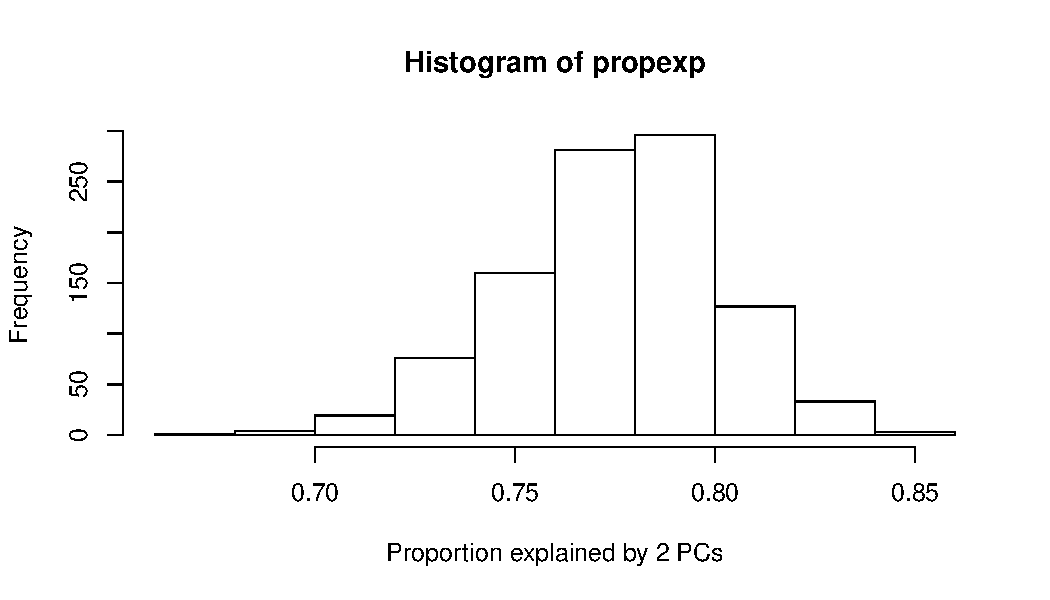
\includegraphics[width=\maxwidth]{figure/p1f-1} \caption[Histogram of Bootstrap]{Histogram of Bootstrap}\label{fig:p1f}
\end{figure}


\end{knitrout}

\paragraph{Problem 2:} This data set contains information about the
chemical composition of wines. Perform PCA and comment on the results.

\paragraph{Solution 2:} For this dataset $n>>p$. However, the units
for the variables are different, which calls for doing PCA on the
correlation matrix. Based on Figure \ref{fig:p2a}, we apply
the log transform on the data to help stabilize it. However, a
comparison with the unlog transformed data indicates that this only
marginally improves the proportion explained. The screeplot in Figure
\ref{fig:p2b} indicates that we should hold onto at least 3 PCs as
well. Four could be appropriate too, if we wanted to explain at least
70\% of the variance. By studying the factor loadings, we can see that
PC1 is largely driven by Total.phenols, Falavanoids and
OD280.OD315 while PC2 is Alcohol.content, Color.Intensity and Proline,
PC3 is As and Alcalinity.in.ash while PC4 divies those with high
Malic.acid and Proantocyanins against those with high Hue and Nonflavanoid.phenols.
\begin{knitrout}
\definecolor{shadecolor}{rgb}{0.969, 0.969, 0.969}\color{fgcolor}\begin{kframe}
\begin{alltt}
\hlstd{data2} \hlkwb{=} \hlkwd{read.csv}\hlstd{(}\hlstr{"wine.csv"}\hlstd{,} \hlkwc{header}\hlstd{=}\hlnum{TRUE}\hlstd{)}
\hlstd{data20} \hlkwb{=} \hlstd{(}\hlkwd{as.matrix}\hlstd{(data2))}
\hlkwd{matplot}\hlstd{(}\hlkwd{t}\hlstd{(data20),}\hlkwc{type} \hlstd{=} \hlstr{"l"}\hlstd{,} \hlkwc{xlab} \hlstd{=} \hlstr{"Variables"}\hlstd{,} \hlkwc{ylab} \hlstd{=} \hlstr{"Wines"}\hlstd{)}
\end{alltt}
\end{kframe}\begin{figure}[H]
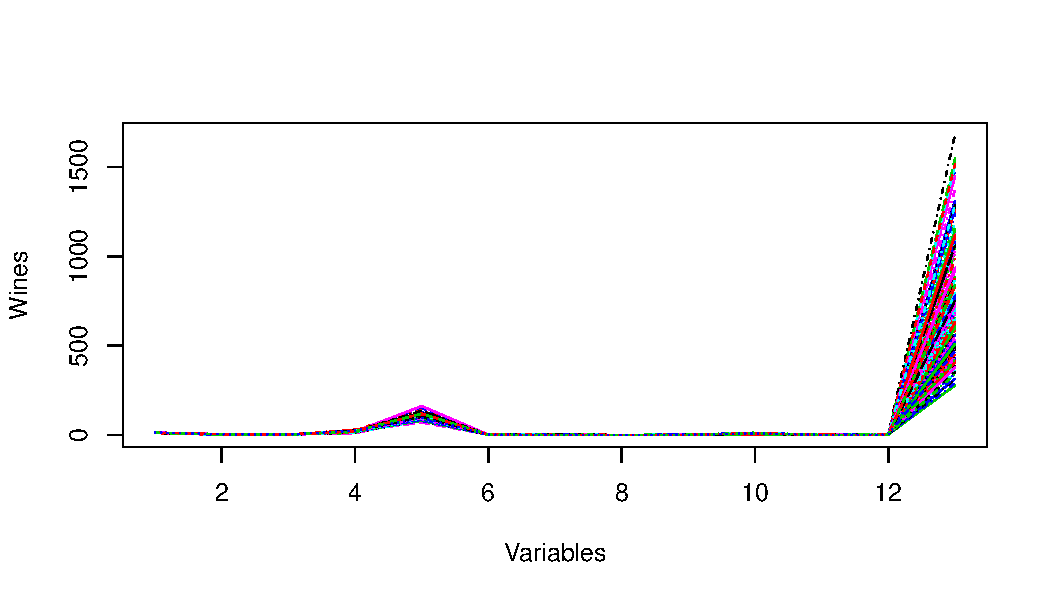
\includegraphics[width=\maxwidth]{figure/p2a-1} \caption[Screeplot]{Screeplot}\label{fig:p2a}
\end{figure}

\begin{kframe}\begin{alltt}
\hlstd{data20} \hlkwb{=} \hlkwd{log}\hlstd{(}\hlkwd{as.matrix}\hlstd{(data2))}
\hlstd{pc21} \hlkwb{=} \hlkwd{prcomp}\hlstd{(data20,} \hlkwc{center} \hlstd{=} \hlnum{TRUE}\hlstd{,} \hlkwc{scale} \hlstd{=} \hlnum{TRUE}\hlstd{)}
\hlkwd{summary}\hlstd{(pc21)}\hlopt{$}\hlstd{importance[,}\hlnum{1}\hlopt{:}\hlnum{4}\hlstd{]}
\end{alltt}
\begin{verbatim}
##                             PC1     PC2      PC3      PC4
## Standard deviation     2.140819 1.65417 1.218038 0.938557
## Proportion of Variance 0.352550 0.21048 0.114120 0.067760
## Cumulative Proportion  0.352550 0.56303 0.677150 0.744910
\end{verbatim}
\begin{alltt}
\hlkwd{summary}\hlstd{(pc21)}\hlopt{$}\hlstd{rotation[,}\hlnum{1}\hlopt{:}\hlnum{4}\hlstd{]}
\end{alltt}
\begin{verbatim}
##                              PC1         PC2         PC3         PC4
## Alcohol.content      -0.10842850  0.47918760 -0.17865648  0.03436658
## Malic.acid            0.24914242  0.21952916  0.19286581 -0.46548550
## As                    0.01891262  0.29984440  0.60322701  0.30925797
## Alcalinity.in.ash     0.24000989 -0.06280937  0.60205834 -0.01609889
## Magnesium            -0.12779786  0.33176191  0.09148971  0.16530774
## Total.phenols        -0.39545612  0.06418244  0.15084280 -0.08133091
## Falavanoids          -0.42757871 -0.03987141  0.16118936 -0.09455543
## Nonflavanoid.phenols  0.29012478 -0.02028423  0.16120235  0.41176889
## Proantocyanins       -0.31688859  0.05267407  0.25031696 -0.43090965
## Color.Intensity       0.09029551  0.51872905 -0.11869307 -0.06840962
## Hue                  -0.33284741 -0.22538876  0.01941531  0.46783535
## OD280.OD315          -0.39359075 -0.13786792  0.16328603 -0.07315717
## Proline              -0.23285697  0.41289943 -0.13285159  0.24335554
\end{verbatim}
\end{kframe}
\end{knitrout}
The screeplot in Figure \ref{fig:p1d} indicates that it is sufficient to hold on to 2 PCs.
\begin{knitrout}
\definecolor{shadecolor}{rgb}{0.969, 0.969, 0.969}\color{fgcolor}\begin{kframe}
\begin{alltt}
\hlkwd{screeplot}\hlstd{(pc21)}
\end{alltt}
\end{kframe}\begin{figure}[H]
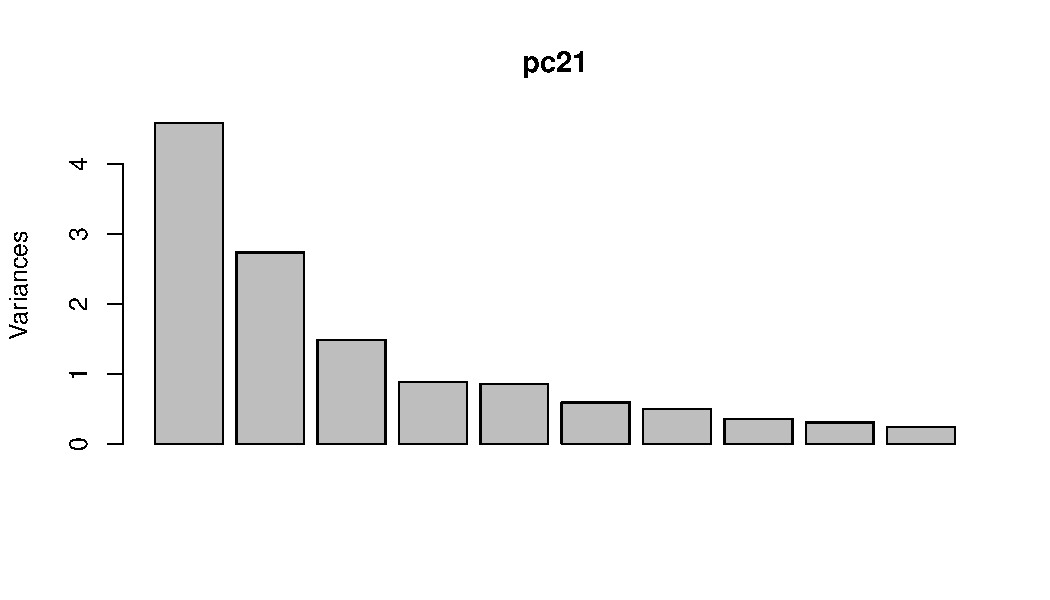
\includegraphics[width=\maxwidth]{figure/p2b-1} \caption[Screeplot]{Screeplot}\label{fig:p2b}
\end{figure}


\end{knitrout}


\begin{knitrout}
\definecolor{shadecolor}{rgb}{0.969, 0.969, 0.969}\color{fgcolor}\begin{kframe}
\begin{alltt}
\hlkwd{biplot}\hlstd{(pc21)}
\end{alltt}
\end{kframe}\begin{figure}[H]
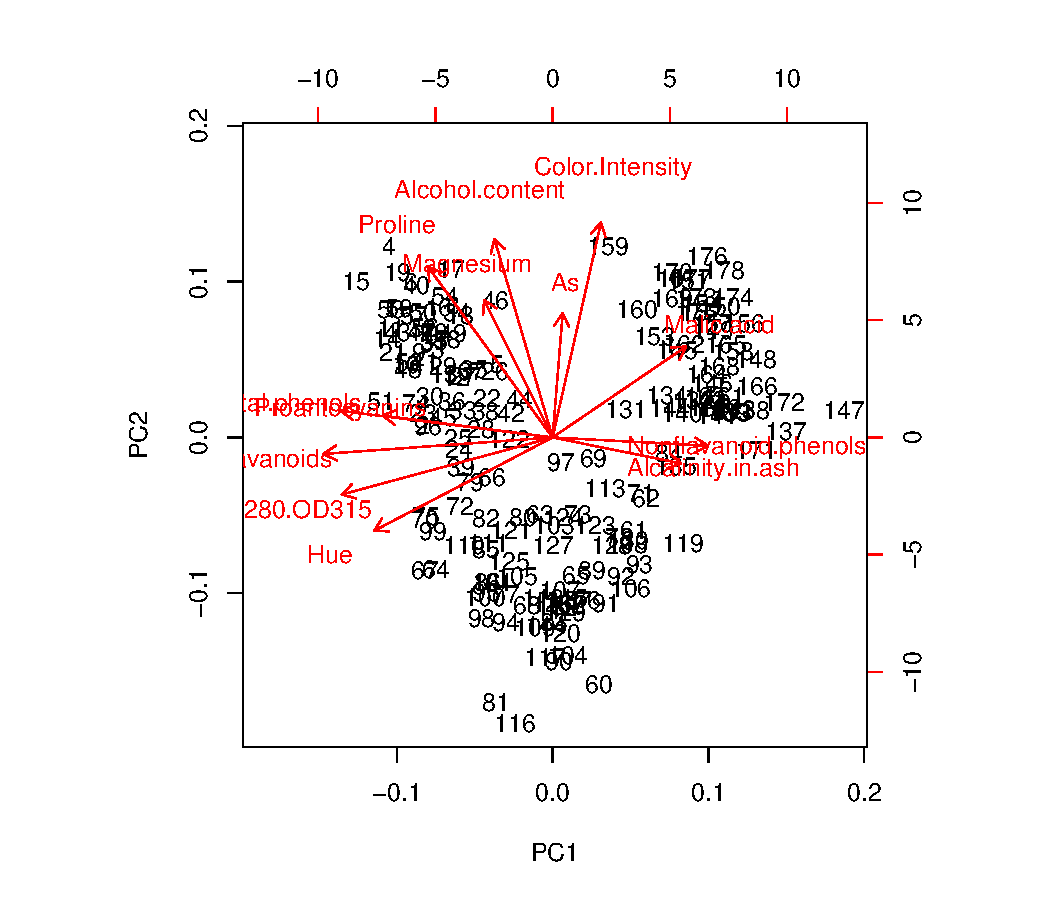
\includegraphics[width=\maxwidth]{figure/p2c-1} \caption[Bi-plot]{Bi-plot}\label{fig:p2c}
\end{figure}


\end{knitrout}

\end{document}
